\input{../preamble}
\input{../usercommands}

\begin{document}

\vspace*{2cm}

{\centerline{\bf\huge AST2000 Lecture Notes}}

\vspace*{1cm}

\newcommand{\PartName}{2B}
\newcommand{\refproblem}[1]{\PartName.\ref{#1}}


{\centerline{\bf\LARGE Part \PartName}}\vspace*{0.25cm}
{\centerline{\bf\LARGE Four vectors and relativistic dynamics}}

\vspace*{1cm}

{\centerline{\underline{\LARGE Questions to ponder before the lecture}}}

\vspace*{1cm}

{\large
\begin{enumerate}
\item A position vector is a vector pointing to a position in 3 dimensions. In relativity it could be useful to include the position in time and make a four dimensional position vector. Would such a vector obey the usual rules for vector aritmetics? (try to think about some simple examples, i.e. of adding position vectors)
\item We have seen that in the special theory of relativity, also the pace of time changes when you move. Could this be interpreted as you having a four-dimensional velocity including a time component of your velocity vector? How could you define such a 4 dimensional velocity?
\item The velocity of an object changes when you change your frame of reference. Does this mean that also momentum and energy are relative quantities? What happens in this case to the law of conservation of energy?
\end{enumerate}

\begin{Figure}%[htb]
\centering
%\begin{center}
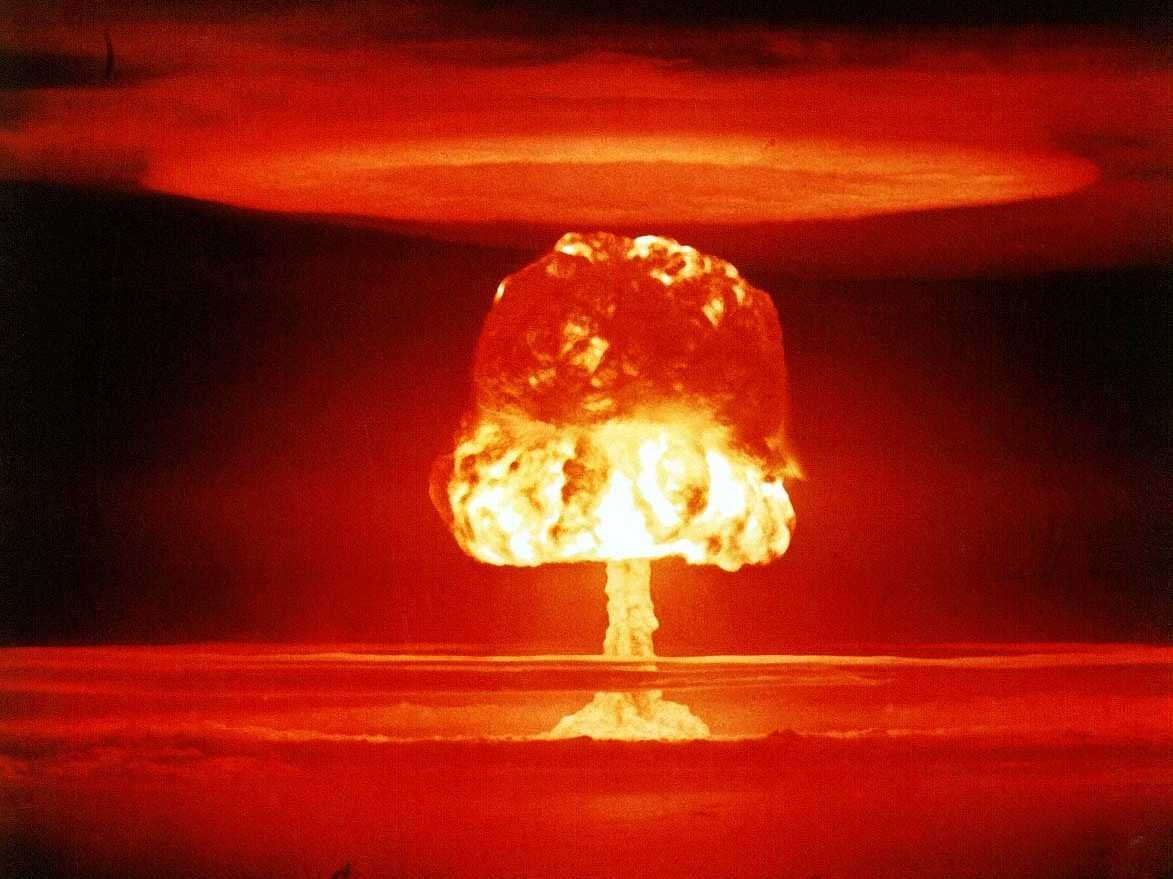
\includegraphics[width=0.8\textwidth]{atomic_bomb.jpg}
%\end{center}
\end{Figure}
%Image: wikipedia commons


\clearpage
\vspace*{2cm}

{\centerline{\bf\huge AST2000 Lecture Notes}}

\vspace*{1cm}

{\centerline{\bf\LARGE Part \PartName}}\vspace*{0.25cm}
{\centerline{\bf\LARGE Four vectors and relativistic dynamics}}


\begin{multicols}{2}

\section{Worldlines}
\label{sect:worldlines}

In the spacetime diagram  in figure \ref{fig:wl} we see the path of a particle (or any object) through spacetime. We see the different positions $(x,t)$ in space and time that the particle has passed through. Such a path showing the points in spacetime that an object passed is called a {\it worldline\label{pg:worldline}}. We will now study two events A and B (on the worldline of a particle) which are separated by a small spacetime interval $\Delta s$. These events could be the particle emitting two flashes of light or the particle passing through two specific points in space. The corresponding space and time intervals between these two events in the laboratory frame are called $\Delta t$ and $\Delta x$. From the figure you see that $\Delta t>\Delta x$. You can see that this also holds for every small spacetime interval along the path. This has to be this way: The speed of the particle at a given instant is $v=\Delta x/\Delta t$. If $\Delta x=\Delta t$ then $v=1$ and the particle travels at the speed of light. That $\Delta t>\Delta x$ simply means that the particle travels at a speed $v<c$ which it must. The worldline of a photon would thus be a line at $45^\circ$ with the coordinate axes. The worldline of any material particle will therefore always make less than $45^\circ$ with the time axis.

Events which are separated by spacetime distances such that $\Delta t>\Delta x$ are called {\it timelike events\label{pg:timelike}}. Timelike events may be causally connected since a particle with velocity $v<c$ would have the possibility to travel from one of the events to the other event. There is a possibility that the second event could have been caused by the first event since it is possible for a signal to travel between the events. Timelike events have positive line elements,
\[
\Delta s^2=\Delta t^2-\Delta x^2>0.
\]

\begin{Figure}%[tbp]
%\begin{center}
\centering
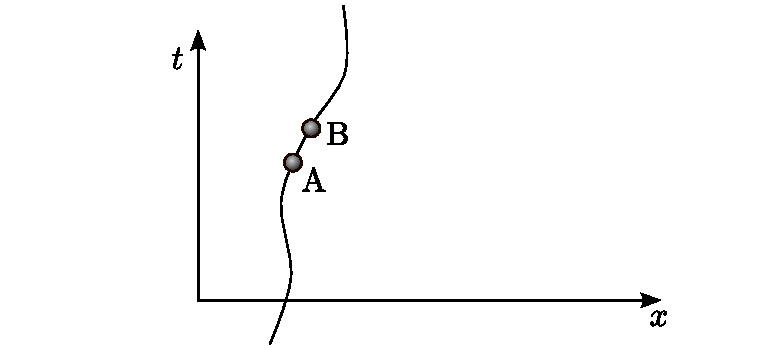
\includegraphics[width=\textwidth]{fig_9-1.pdf}
\captionof{figure}{The worldline, the trajectory of a particle in a spacetime diagram. Two events A and B along the path of the particle have been marked.\label{fig:wl}}
%\end{center}
\end{Figure}


Events for which $\Delta t=\Delta x$ are called {\it lightlike events\label{pg:lightlike}}. Only a particle traveling at the speed of light ($v=\Delta x/\Delta t=1$) could travel from the first event to the second. Lightlike events have zero spacetime interval,
\[
\Delta s^2=\Delta t^2-\Delta x^2=0.
\]
Note one consequence of this: Remember that the proper time interval $\Delta \tau^2$ equals the spacetime interval $\Delta s^2$. Thus, photons always have $\Delta \tau=0$, the wristwatch attached to a photon would not change. Photons and other particles traveling at the speed of light do not feel the effect of time.

Events for which $\Delta x>\Delta t$ are called {\it spacelike events\label{pg:spacelike}}. For these events, the spatial component of the distance is larger than the time component. No worldline could ever connect two spacelike events as it would require a particle to travel faster than light. Thus, spacelike events are not causally connected. The first event could not have caused the second. The spacetime interval for spacelike events is negative,
\[
\Delta s^2=\Delta t^2-\Delta x^2<0.
\]

\begin{Figure}%[tbp]
%\begin{center}
\centering
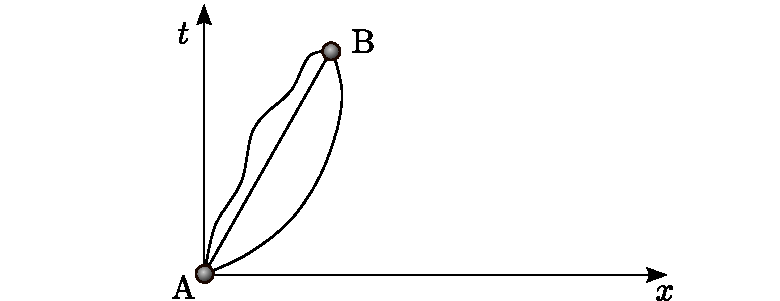
\includegraphics[width=\textwidth]{fig_9-2.pdf}
\captionof{figure}{Different worldlines connecting the two events A and B.\label{fig:ab}}
%\end{center}
\end{Figure}

In figure \ref{fig:ab} we see two events A and B and three different worldlines between these events. These events could be a car passing position $x_A$ and position $x_B$ in the laboratory frame. In the spacetime diagram we see three worldlines each corresponding to a car. The straight worldline must correspond to a car driving with constant speed $v=\Delta x/\Delta t=\mathrm{constant}$. The two other worldlines must correspond to cars accelerating (changing their speed and thereby changing the slope of the worldline) along the way from $x_A$ to $x_B$, but all cars reach point $x_B$ at the same time (event B). All cars also passed point $x_A$ at the same time (event A). Same time here means 'same time' for all frames of reference: all the cars meet at event A and B, so if they meet simultaneously in one frame of reference they must meet simultaneously in all other frames of reference (did you get this? If not, read the sentences again!). 

\pagebreak[2]

We will now ask a question which answer may seem obvious in this case, but which might not be so obvious in other situations. The question is: Given a particle (or a car) going from event A to event B. If this particle is in free float (in special relativity this means that no forces act on the particle), which worldline will the particle take between event A and event B? Looking back at figure \ref{fig:ab} we see three possible worldlines, but in fact there is an infinite number of possible worldlines connecting the two events. The obvious answer in this case is that it will follow a straight line in spacetime, i.e.\ the straight worldline corresponding to constant velocity. This is just a modern way of saying Newton's first law: A body which is not under the influence of external forces will continue moving with constant velocity. But is there a deeper principle behind? In the theory of relativity there is, and this principle is called the {\it principle of maximal aging\label{pg:maximalaging}}. This is a fundamental principle in the special as well as in the general theory of relativity.

The principle of maximal aging says that a particle in free float (no forces act on the particle) will follow the worldline which corresponds to the longest possible proper time interval between the two events. We remember that proper time is the wristwatch time\label{pg:wristwatchtime}, the time measured on the clock attached to the particle. So let different particles take different paths in spacetime between the two events. Attach a wristwatch to each of the particles. At event B, you look at the time interval between event A and B measured on the wristwatch of each of the particles. The particle which measures the longest proper time, i.e.\ the particle with the wristwatch which made most ticks during the trip from event A to event B, is the particle taking the path that a particle in free-float would take. 

How do we calculate the proper time interval that a given particle takes from event A to event B? The clue is to remember that the proper time interval $\Delta\tau$ between two events equals the spacetime interval, or the total length of the path in spacetime $\Delta s$ taken between the two events. For the worldline of a particle with constant velocity, we know that the distance in spacetime traveled from event A to event B is just $\Delta s=\sqrt{\Delta t^2-\Delta x^2}$ where $\Delta x$ and $\Delta t$ are space and time intervals measured in an arbitrary frame of reference. To measure the total spacetime interval along the worldline of a particle which does not move with constant velocity, we need to break the path up into small path lengths $ds$. This path length is so small that we can assume the velocity to be constant during the time it takes to travel this interval in spacetime. We can thus write $ds=\sqrt{dt^2-dx^2}$ where $dx$ and $dt$ are the corresponding small space and time displacement measured in the arbitrary frame of reference. To obtain the total length of the path in spacetime traveled between two events A and B, we need to integrate all these tiny spacetime intervals $ds$ giving
\begin{equation}
\label{eq:ds}
\Delta s=\int_A^B\sqrt{dt^2-dx^2}.
\end{equation}
This equals measuring the length $s$ of a curved path between two points A and B in the x-y plane:
\[
\Delta s=\int_A^B\sqrt{dx^2+dy^2}.
\]
Note again a huge difference here: The minus sign in the spacetime interval. We know from Euclidean geometry that the shortest path $s$ between two points A and B in the plane, is the straight line. The minus sign in the line element for Lorentz geometry gives rise to the opposite result (which we will not derive here): The \emph{longest} path $s$ between two events A and B in spacetime is the straight worldline. Therefore, if we measure the length of the spacetime path for all the three worldlines in figure \ref{fig:ab} using the integral in (\ref{eq:ds}), we find that the longest path in spacetime is the straight worldline, i.e.\ the worldline of the car driving with constant velocity. Remember again that the length of the spacetime interval $\Delta s$ equals the total proper time $\Delta\tau$ measured on the wristwatch of the particle. So the longest proper time interval between two events is measured on the particle taking the straight line in spacetime, i.e.\ the particle which has constant velocity. We have just deduced Newton's first law from the principle of maximal aging. When we come to the general theory of relativity, we will see that the spacetime geometry and hence the form of the line elements $\Delta s$ is different in a gravitational field. We will need the principle of maximal aging to tell us how a free float particle is moving in this case. 

\begin{figure*}
\fcolorbox{black}{yellow}{\parbox{\dimexpr \linewidth-2\fboxsep-2\fboxrule}{
\begin{minipage}{0.5\textwidth}%{\dimexpr\linewidth-2\fboxsep-2\fboxrule}\parskip=6pt
{\small
\fontfamily{bch}\selectfont
\vspace*{-2.2cm}\hspace*{-0.15cm}\fcolorbox{black}{black}{\bf\color{white} Fact sheet:\color{black}} 
An example of a light cone, the three-dimensional surface of all possible light rays arriving at and departing from a point in spacetime. Here it is depicted with one spatial dimension suppressed. In general, there are three types of curves in spacetime: 1) Time-like curves, with a speed less than the speed of light. These curves must fall within a cone defined by light-like curves. 2) Light-like curves, having at each point the speed of light. They form a cone in spacetime, dividing it into two parts. 3) Space-like curves, falling outside the light cone. (Figure: Wikipedia)
}
\end{minipage}%\hspace*{0.5cm}
\ \ \ \ \ \ \begin{minipage}{0.4\textwidth}
\centering
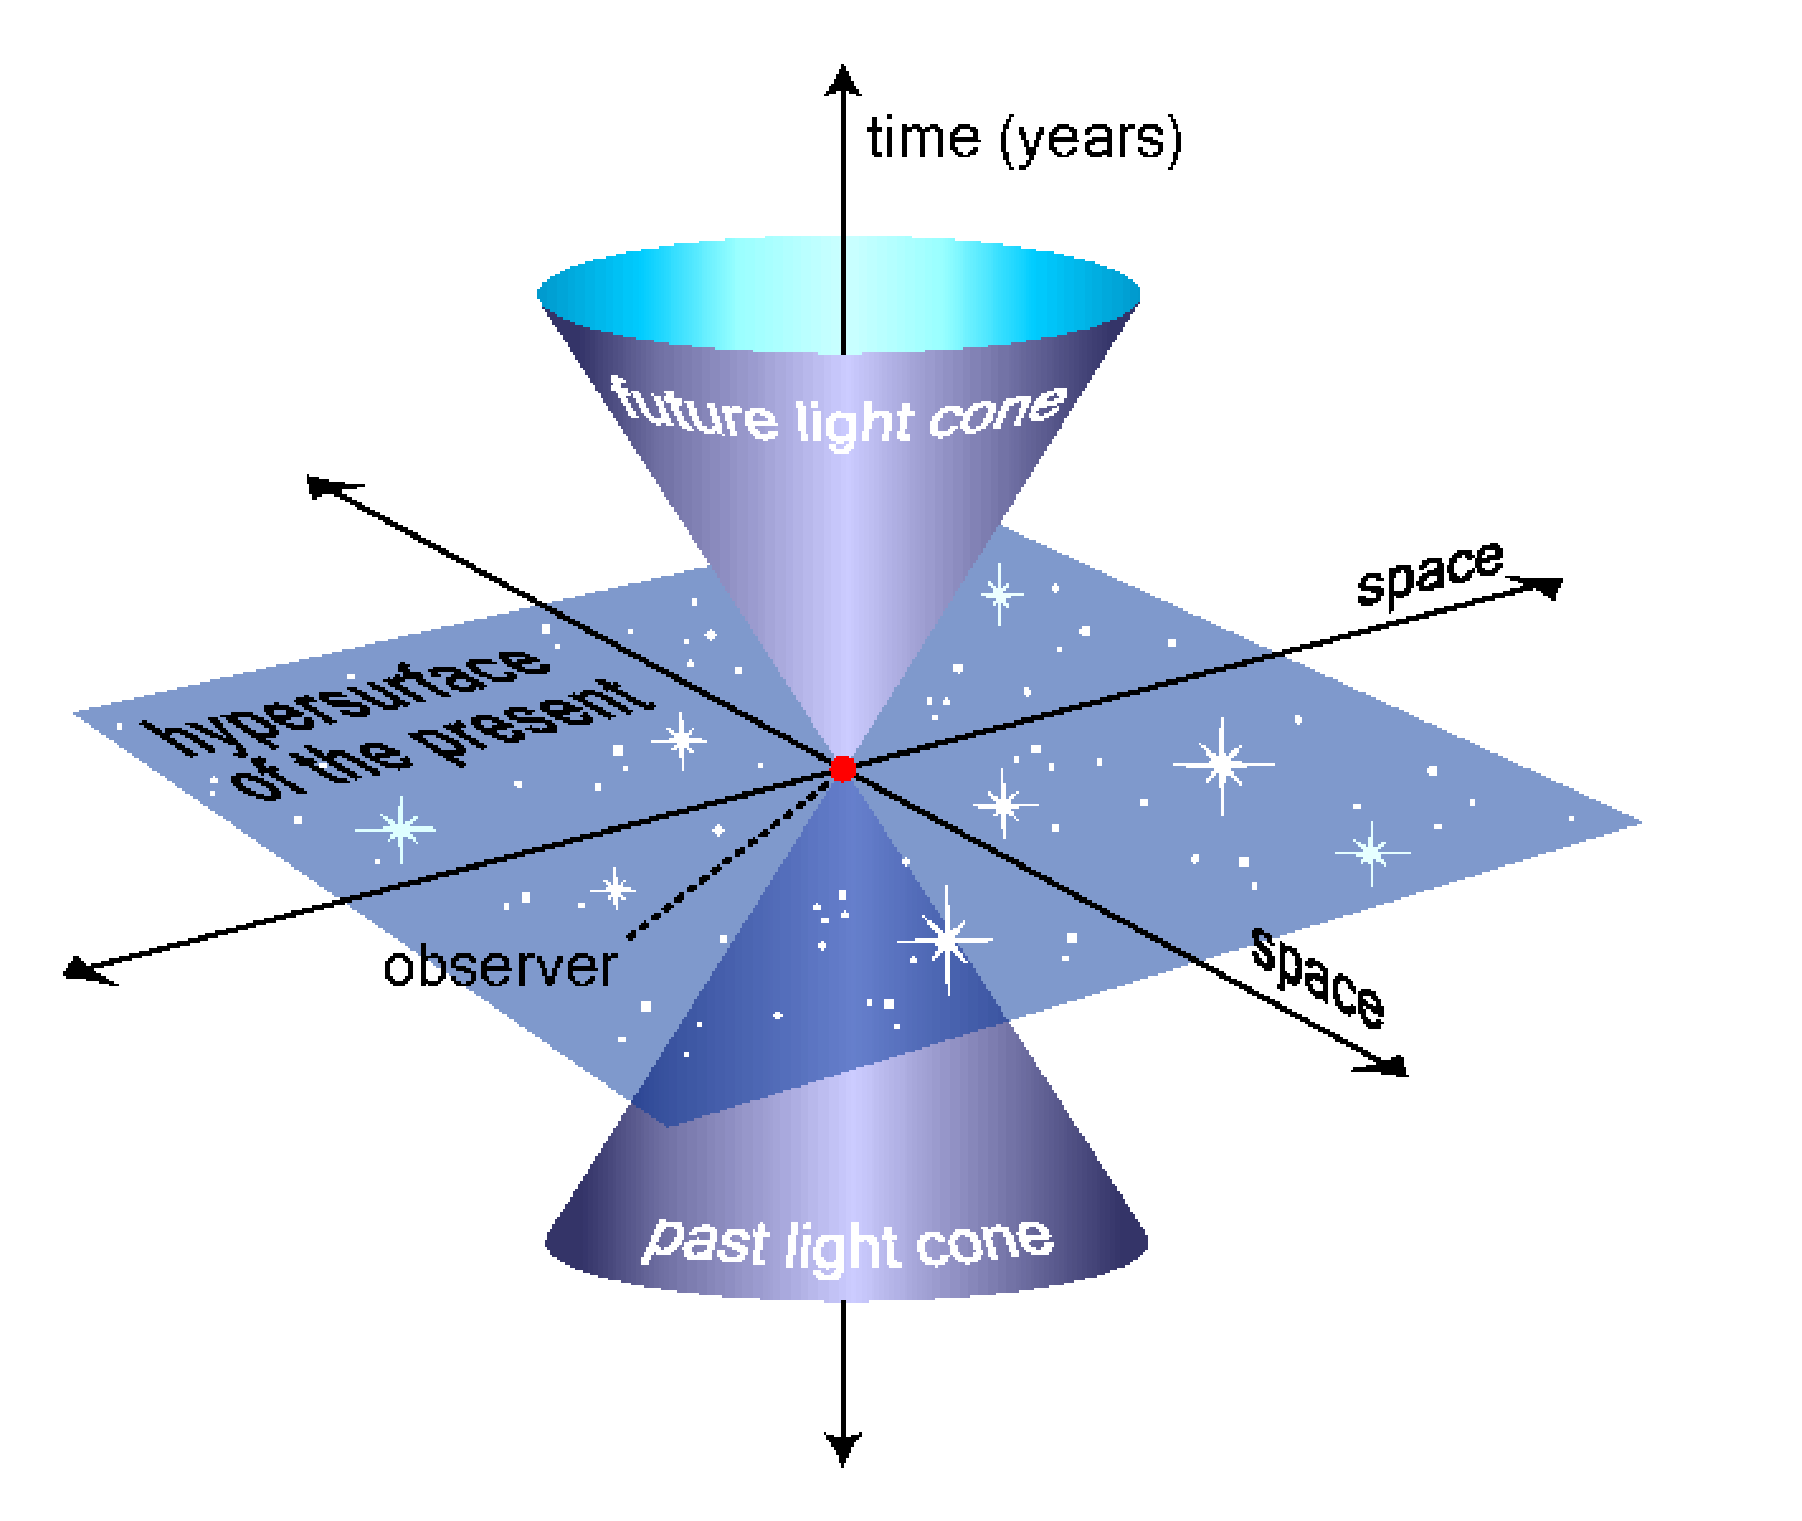
\includegraphics[width=\textwidth,height=0.25\textheight]{lightcone_SR_Wiki.pdf}
%\end{wrapfigure}
%\end{center}
%\end{figure*}
\end{minipage}
}}
\end{figure*}


\section{Four-vectors}
\label{sect:fourvectors}

So far we have used three dimensional vectors to determine a position or event in space. A generalized way way of writing a vector is as followed
\[
\vec{x}=(x_1,x_2,x_3),
\]
which can potentially be the three spatial dimensions. A 4-vector is similarly defined, giving the position of an \emph{event} in four dimensional spacetime as
\[
r=(x_0,x_1,x_2,x_3).
\]
Any and all 4-vector like $r$ are required to transform all non invariant physical quantities (like time) from one frame of reference to another through the given matrix multiplication
\[
\begin{pmatrix}
t' \\
x_1' \\
x_2' \\
x_3'  
\end{pmatrix}
=
\begin{pmatrix}
\gamma&-v\gamma&0&0\\
-v\gamma&\gamma&0&0\\
0&0&1&0\\
0&0&0&1
\end{pmatrix}
\begin{pmatrix}
t \\
x_1 \\
x_2 \\
x_3 \\
\end{pmatrix}.
\]
If there are cases where some of the physical non invariant quantities doesn't transform through and only through the matrix multiplication the vector is \textbf{NOT} a 4-vector.

The matrix multiplication corresponds to the Lorentz transformation from the previous lecture notes (check yourself). For those of you liking linear algebra, the matrix multiplication can be thought of as a type of coordinate mapping between different coordinate systems (or reference frames) using the Lorentz transformation.

For components of a normal three dimensional vector, we use Latin letters, typically $i$ and $j$,  for the indices: The components of $\vec{x}$ are $x_i$ where $i$ goes from 1 to 3. For the components of a 4-vector, we use Greek indices, typically $\mu$ and $\nu$. The components of a four-vector $r$ are $r_\mu$ where $\mu$ run from 0 to 3, 0 being the time component. If we wish to separate the time and space part of a four-vector we might also write it as $r=(t,x_i)$ where $x_i$ refers to all three spatial components.

The matrix multiplication introduced earlier can be written as
\[
r_\mu'=\sum_{\nu=0}^3c_{\mu\nu}r_\nu,
\]
where $c_{\mu\nu}$ is the matrix above. This is the equation which transforms any four-vector from one frame of reference to another. We will now write this equation using the so-called Einstein conventions. Which will be covered more thoroughly in future courses, but for now will save you from a lot of writing. Instead of writing the sum symbol, we simply say that when two factors in a term contain the same index, there is an implicit sum over this index. If the index is Latin, then there is a sum over the three spatial dimensions, if the index is Greek, there is a sum over the three spatial dimensions plus time. Using this convention we can write the previous equation simply as
\begin{formbox}
\begin{equation}
\label{eq:lorentz}
r_\mu'=c_{\mu\nu}r_\nu
\end{equation}
\end{formbox}
which is the formal mathematical definition of a 4-vector.

It can be shown that four-vectors follow the normal rules for summations and subtractions (see exercise 2). We will now look at the scalar product. For three dimensional vectors, the usual scalar product can be written as,
\[
\vec{x}\cdot\vec{y}=\sum_{i=1}^3x_iy_i=x_iy_i,
\]
where the Einstein convention was used in the last expression. We can also define a scalar product for four-vectors. Instead of writing a dot between the vectors, one usually writes the scalar product with one upper index and one lower index,
\[
x^\mu y_\mu=x_0y_0-x_iy_i.
\]
One index $\mu$ is written high and the other low to show that this is the scalar product and \emph{not} a normal sum. Note that the scalar product is defined with a minus sign in front of the spatial part. If we had written both indices low, this would mean,
\[
x_\mu y_\mu=x_0y_0+x_iy_i,
\]
using the Einstein summation convention. This is different from the scalar product. It should be clear where the minus sign comes from, consider a spacetime interval $\Delta x_\mu$ (a spacetime interval is an interval between two points $x_\mu^1$ and $x_\mu^2$ in time and space such that $\Delta x_\mu=x_\mu^1-x_\mu^2=(\Delta t,\Delta x,\Delta y,\Delta z)$). The scalar product of a spacetime interval with itself gives,
\[
\Delta x^\mu\Delta x_\mu=\Delta t^2-\Delta x^2=\Delta s^2
\]
(assuming $\Delta y=\Delta z=0$). The result is the {\it scalar\label{pg:scalar}} $\Delta s^2$. A scalar is a quantity which is invariant, which has the same value in all frames of reference. We already knew that the spacetime interval $\Delta s^2$ is a scalar (where did we learn this?). For infinitesimal distances between events, we may write this as,
\[
ds^2=dx^\mu dx_\mu.
\]

We learned above that a four vector\label{pg:fourvector} is a vector which transforms according to the Lorentz transformation (equation \ref{eq:lorentz}) when changing from one frame of reference to another frame of reference having velocity $v$ with respect to the first. This has an important consequence: You cannot choose 4 numbers on random, put them together and call it a 4-vector! The numbers entering in a four-vector need to be physical quantities which are such that the 4-vector transforms accoring to equation \ref{eq:lorentz}. We thus need to take care when performing mathematical operations with 4-vectors: The result may not necessarily be a 4-vector.

As an example we will now investigate what happens with a 4-vector when multiplying it with some random physical quantity. Say that you for some reason need to multiply a spacetime distance $\Delta r_\mu=(\Delta t,\Delta x,\Delta y,\Delta z)$ with the corresponding time interval $\Delta t$ forming 
\[
\Delta u_\mu=\Delta t\Delta r_\mu.
\]
Is $\Delta u_\mu$ a 4-vector? We can easily check this by checking whether it transforms according to equation \ref{eq:lorentz} when changing frame of reference. We therefore need to find $\Delta u_\mu'$ as
\[
\Delta u_\mu'=\Delta t'\Delta r_\mu'
\]
and test if equation \ref{eq:lorentz} is satisfied.

We know that $\Delta r_\mu$ follows this transformation. We also now that $\Delta t'=(1/\gamma)\Delta t$ when changing frame of reference. We thus have for $\Delta u_\mu'$ in a new frame of reference
\[
\Delta u_\mu'=\Delta t'\Delta r_\mu'=(1/\gamma)\Delta tc_{\mu\nu}\Delta r_\nu=(1/\gamma) c_{\mu\nu}\Delta u_\nu.
\]
Because of the factor $1/\gamma$ we see that $\Delta u_\mu$ does not transform according to equation \ref{eq:lorentz} and $\Delta u_\mu$ is therefore NOT a 4-vector. We thus cannot multiply a 4-vector with a time interval and obtain a 4-vector.

A four-vector which is multiplied by a scalar however, is itself a four-vector. If instead of multiplying $\Delta r_\mu$ with $\Delta t$, we multiply it with the corresponding spacetime interval $\Delta s$ we get
\[
\Delta u_\mu=\Delta s\Delta r_\mu.
\]
Transforming to a different frame of reference we have again $\Delta r_\mu'=c_{\mu\nu}\Delta r_\nu$ since $\Delta r_\mu$ is a four-vector and $\Delta s'=\Delta s$ since $\Delta s$ is a scalar. We thus have
\[
\Delta u_\mu'=\Delta s'\Delta r_\mu'=\Delta sc_{\mu\nu}\Delta r_\nu=c_{\mu\nu}\Delta u_\nu
\]
which does follow equation \ref{eq:lorentz}. In this case $\Delta u_\mu$ is a four-vector. We thus have generally that when $A_\mu$ is a four vector and $f$ is a scalar, the product
\[
B_\mu=fA_\mu,
\]
is a 4-vector.


\section{Four-velocity}
\label{sect:fourvel}

Can we define a four dimensional velocity $V_\mu$, that is, a four dimensional vector showing the direction of motion in spacetime of a particle with coordinates $x_\mu$? By analogy to normal three dimensional velocity, the four-velocity $V_\mu$ should be the the rate of change of the position vector $x_\mu$. A natural choice would be $dx_\mu/dt$, but this is not a four-vector: As we discussed above, $\Delta t$ or $dt$ is not a scalar, it has different values in different frames of reference. Thus $dx_\mu/dt$ does not transform as a 4-vector, i.e.\ you cannot use the Lorentz transformation to transform it from one frame of reference to another. But in order to have velocity, we need the rate of change with respect to some time interval $\Delta t$. Which measure of time can we use?

Remember that proper time $\tau$ is a scalar, it is defined as the time observed on the wristwatch of an observer. All observers will measure the same time interval $\Delta\tau$ between two events (how do they measure $\Delta\tau$?). Consider the example with the train and observer P who is jumping up and down. Measured on the wrist watch of observer P, one jump takes one second, thus one second of proper time for the frame of reference of the train. According to observer O's wristwatch, the jump takes 1.7 seconds, but this is not the proper time for the train (remember the definition of proper time!). But observer O can take his binoculars and read of the time between each jump on observer P's wristwatch. He will then find, in agreement with observer P, that in proper time units for the train, each jump takes one second. 

Note that proper time needs to be defined with respect to some frame of reference (in this case the train), but once this is defined, everybody agrees on the proper time interval between two events taking place at the same spot in that frame. In the case of four-velocity, there is no doubt about which proper time we are speaking about: Four-velocity is the velocity of a particle or an object (for instance a train) and the proper time $\Delta\tau$ which we use to define four velocity is the time measured in the rest frame of this object. So four-velocity\label{pg:fourvelocity} can be defined as
\[
V_\mu=\frac{dx_\mu}{d\tau}.
\]
Let us find the length (absolute value) of the four-velocity (the square root of the scalar product of the vector with itself). The square of the length is (as for normal vectors) given by
\[
V_\mu V^\mu=\frac{dx_\mu}{d\tau}\frac{dx^\mu}{d\tau}=\frac{dx_\mu dx^\mu}{d\tau^2}=\frac{ds^2}{d\tau^2}=\frac{d\tau^2}{d\tau^2}=1.
\]
(did you understand every step here?)
Taking the square root of this we still get 1. The length of the four-velocity is thus always one. Remember that a velocity of one means the velocity of light. All particles move with the velocity of light in spacetime! For each proper time interval $\Delta\tau$ a particle moves an equal interval $\Delta s$ in spacetime.

\begin{Figure}%[tbp]
%\begin{center}
\centering
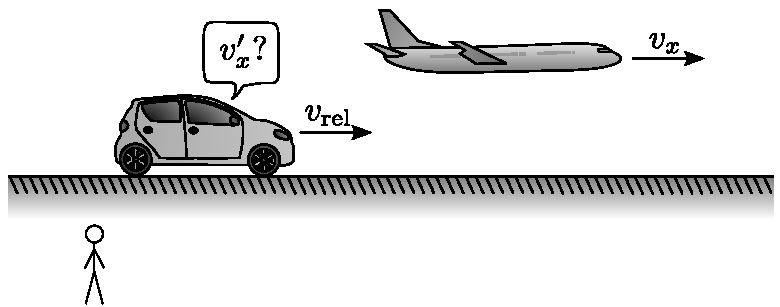
\includegraphics[width=\textwidth]{fig_9-3.pdf}
\captionof{figure}{The observer on the ground measuring a velocity $v_x$ for the airplane, wondering which velocity $v_x'$ the driver of the car measures for the same airplane.\label{fig:vx}}
%\end{center}
\end{Figure}

We can write the four-velocity in terms of normal 3-velocity as
\begin{formbox}
\begin{align*}
&V_\mu=(\frac{dt}{d\tau},\frac{dx_i}{d\tau})\\
&=(\frac{dt}{d\tau},\frac{dt}{d\tau}\frac{dx_i}{dt})=\frac{dt}{d\tau}(1,\vec{v})=\gamma(1,\vec{v})
\end{align*}
\end{formbox}
where we have used that $\Delta t/\Delta\tau=dt/d\tau=\gamma$ from the previous lecture notes (go back and check how you derived this, it is important!)(\textbf{Vi gjør aldri dette i part2A!}). Now we are ready to answer a question that has bothered us all the time since we learned about the Lorentz transformations: We know how to transform between coordinates $(x,t)$  and $(x',t')$ in two different frames of reference. But how do you transform a velocity $v_x$ from one frame to the other? Say that you stand on the ground and look at a passing airplane. You measure the velocity of the airplane along the x-axis to be $v_x$. A car is passing you on the street with velocity $v_\mathrm{rel}$ along the same x-axis and you note that the driver is also watching the airplane. You start to wonder which velocity $v_x'$ that the driver is measuring for the airplane. The situation is depicted in figure \ref{fig:vx}. In normal non-relativistic physics you know that the answer should read $v_x'=v_x-v_\mathrm{rel}$, but we have learned that this does not work for velocities close to the velocities of light (for instance, look back at the Michelson-Morley experiment). Assuming that there are no motions in the $y$ and $z$ direction, we can now write the four velocity of the airplane from our laboratory frame as $V_\mu=\gamma(1,v_x)$ and from the car as $V_\mu'=\gamma'(1,v_x')$ where $\gamma=1/\sqrt{1-v_x^2}$ and $\gamma'=1/\sqrt{1-(v_x')^2}$. We know that four-velocity is a four-vector and that four-vectors by definition transform from one frame of reference to the other under the Lorentz transformation,
\begin{formbox}
\[
V_\mu'=c_{\mu\nu}V_\nu,
\]
\end{formbox}
or written in terms of matrices as
\begin{formbox}
\[
\begin{pmatrix}
\gamma'\\
\gamma'v_x'\\
\gamma'v_y'\\
\gamma'v_z'
\end{pmatrix}
=
\begin{pmatrix}
\gamma_\mathrm{rel}&-v_\mathrm{rel}\gamma_\mathrm{rel}&0&0\\
-v_\mathrm{rel}\gamma_\mathrm{rel}&\gamma_\mathrm{rel}&0&0\\
0&0&1&0\\
0&0&0&1
\end{pmatrix}
\begin{pmatrix}
\gamma\\
\gamma v_x\\
\gamma v_y\\
\gamma v_z
\end{pmatrix}
\]
where $\gamma_\mathrm{rel}=1/\sqrt{1-v_\mathrm{rel}^2}$.
\end{formbox}
From this matrix equation, we obtain two equations for the velocity $v_x$ and $v_x'$,
\begin{align*}
\gamma'&=(\gamma_\mathrm{rel}-v_\mathrm{rel}\gamma_\mathrm{rel}v_x)\gamma\\
\gamma'v_x'&=(-v_\mathrm{rel}\gamma_\mathrm{rel}+\gamma_\mathrm{rel}v_x)\gamma.
\end{align*}
Dividing the second equation by the first, we obtain
\begin{formbox}
\begin{equation}
\label{eq:vel}
v_x'=\frac{v_x-v_\mathrm{rel}}{1-v_\mathrm{rel}v_x},
\end{equation}
\end{formbox}
which is the Lorentz transformation for velocities. Note that when the speed of the airplane approaches the speed of light, $v_x\rightarrow1$ then $v_x'\rightarrow1$ showing that the laboratory observer and the observer in the car will both measure the speed of light for the airplane. This solves the weird result obtained by Michelson and Moreley: The speed of light is the same from all frames of reference.

\section{Relativistic momentum and energy}
\label{sect:energy}

What about momentum and energy? We have learned that the velocity $v$ of an object as measured from two different frames of reference transform according to the Lorentz transformation (equation \ref{eq:vel}). This must necessarily have consequences for how we measure momentum $p=mv$ and energy $E=1/2mv^2$ from two different frames of reference. There must be some corresponding Lorentz transformations for momentum and energy. We have learned a simple and easy recipe for finding the transformation equations between different frames: Construct a four-vector and use the transformation properties for four-vectors. This worked for velocity so let's try with momentum and energy.

We start with momentum. In order to construct a four-vector $P_\mu$ for momentum, let's try a form which is as similar as possible to the Newtonian form $\vec{p}=m\vec{v}$. Rest mass (the mass measured in the rest frame of the object) is a scalar quantity, so
\[
P_\mu=mV_\mu
\]
is a four-vector. Using that $V_\mu=\gamma(1,\vec{v})$, we can write momentum as
\begin{formbox}
\[
P_\mu=m\gamma(1,\vec{v})=\gamma(m,\vec{p}),
\]
\end{formbox}
where $\vec{p}$ is the Newtonian momentum. Taking the spatial part of this equation we see that relativistic momentum can be written in three dimensions simply as
\begin{equation}
\label{eq:p}
\vec{p}_\mathrm{relativistic}=\gamma m \vec{v},
\end{equation}
where $\vec{v}$ is the normal 3-velocity of an object. What is the meaning of the time component $P_0=\gamma m$ of the momentum 4-vector? In order to investigate this let us write it in the Newtonian limit. For $v<<1$ (velocity much lower than the velocity of light) we can make a Taylor expansion in $v$,
\[
P_0(v)=P_0(v=0)+\frac{dP_0}{dv}(v=0)v+\frac{1}{2}\frac{d^2P_0}{dv^2}(v=0)v^2,
\]
where the derivatives taken at $v=0$ are (check it!) $P_0(v=0)=m$, $dP_0/dv(v=0)=0$ and $d^2P_0/dv^2(v=0)=m$. We get
\[
P_0=m+\frac{1}{2}mv^2.
\]
The last term is just the expression for Newtonian kinetic energy. The first term is the {\it rest energy} of a particle, converted to normal units it can be written as the more well known  $E=mc^2$. The rest energy is the energy of a particle at rest, it is the energy in the mass of the particle. Thus, the time component of the momentum four-vector is relativistic energy,
\begin{equation}
\label{eq:E}
E_\mathrm{relativistic}=m\gamma,
\end{equation}
which in the Newtonian limit reduces to the Newtonian kinetic energy plus an energy term which did not exist in Newtonian physics, the energy of the mass of the particle. So the 4-vector $P_\mu$ is not just a momentum 4-vector, it is {\it the momentum-energy 4-vector} which time component is energy and space component is momentum. It means that energy and momentum are related in the same way as space and time are. In the same manner as we talk about spacetime, indicating that space and time are basically two aspects of the same thing, we can call energy and momentum collectively as {\it momenergy\label{pg:momenergy}}. The four-vector $P_\mu$ is simply the {\it momenergy four-vector}.

What is the length of the momenergy four-vector? Using that $P_\mu=mV_\mu$ we have for the square of the length
\[
P_\mu P^\mu=m^2V_\mu V^\mu=m^2.
\]
The length is the square root of $m^2$ which is $m$. The length of the momenergy four-vector is an invariant and it is thus simply the mass. We have seen that we can write $P_\mu=\gamma(m,\vec{p})$ giving (using equations \ref{eq:p} and \ref{eq:E})
\[
P_\mu=(E_\mathrm{relativistic},\vec{p}_\mathrm{relativistic}).
\]
From now on we will drop the subscript 'relativistic' and always refer to the relativistic energy and relativistic momentum using $E$ and $p$. But how can we be so sure? How can we know that this is the correct expression for energy and momentum? What is the criterion for a quantity to be energy or momentum? We know that energy and momentum are conserved quantities. The total energy and momentum of particles after a collision should always be the same as the total energy and momentum before the collision. So this is easy to check: Measure the total energy and momentum of particles before and after a collision, if they are the same we have found the correct expressions for momenergy. This has been tested thousands of times in particle accelerators with particles moving close to the speed of light. It turns out that the Newtonian energy and momentum are \emph{not} conserved in these collisions. The relativistic energy and momentum defined as we have done above however, \emph{are} conserved.

By now we have got used to measure time and space in the same units and therefore we have also got used to add these quantities $\Delta x+\Delta t$ without hesitating. We see that the result of measuring time and space in the same units is that momentum and energy are also measured in the same units, the units of mass. We remember that since space and time are measured in the same units, the speed $v$ is a dimensionless number. The factor $\gamma$ is clearly also dimensionless, so the momentum $p=m\gamma v$ can be measured in the units of mass (kg). The same goes for energy $E=m\gamma$, which also has dimension mass. So both energy and momentum are measured in kg and these quantities can therefore be added, just as we can add intervals in time and distances in space. The momenergy four-vector is $P_\mu=(E,\vec{p})$, taking the scalar product we have (remembering the result above that the length of $P_\mu$ is just $m$),
\[
P_\mu P^\mu=E^2-p^2=m^2,
\]
we can thus write energy in terms of momentum as
\[
E=\sqrt{m^2+p^2}.
\]
A photon is massless, so for photons this relation is just
\[
E=p,
\]
or by using normal units $E=pc$ which is a more known form of this expression. The energy of a photon can also be written as
\begin{equation}
E=h\cdot f=\dfrac{h}{\lambda}
\end{equation}
where $f$ is the frequency, $h$ is the Planck constant in unites dived by $c$ and $\lambda$ is the wavelength.

We return to the above example with the airplane and the passing car. You measure the relativistic energy and momentum of the airplane from the laboratory frame (the ground) and you wonder what energy and momentum the driver of the car measures for the same airplane. The momenergy four-vector is a four-vector which means that it can be transformed from one frame of reference to the other by the Lorentz transformation,
\begin{formbox}
\[
P_\mu'=c_{\mu\nu}P_\nu,
\]
\end{formbox}
or in matrix form (remember that there were no movements in the $y$ and $z$ direction)
\begin{formbox}
\[
\begin{pmatrix}
E'\\
p_x'\\
p_y'\\
p_z'
\end{pmatrix}
=
\begin{pmatrix}
\gamma_\mathrm{rel}&-v_\mathrm{rel}\gamma_\mathrm{rel}&0&0\\
-v_\mathrm{rel}\gamma_\mathrm{rel}&\gamma_\mathrm{rel}&0&0\\
0&0&1&0\\
0&0&0&1
\end{pmatrix}
\begin{pmatrix}
E\\
p_x\\
p_y\\
p_z
\end{pmatrix}
\]
\end{formbox}

Giving the following transformation equations for momentum and energy
\begin{align*}
E'&=\gamma_\mathrm{rel}E-v_\mathrm{rel}\gamma_\mathrm{rel}p_x\\
p_x'&=\gamma_\mathrm{rel}p_x-v_\mathrm{rel}\gamma_\mathrm{rel}E
\end{align*}
where $v_\mathrm{rel}$ is the relative velocity between the two frames of reference, the observer on the ground and the car (see figure \ref{fig:px}). 

\begin{Figure}%[tbp]
%\begin{center}
\centering
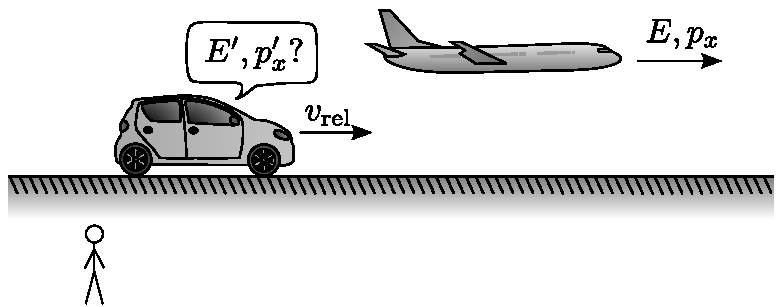
\includegraphics[width=\textwidth]{fig_9-4.pdf}
\captionof{figure}{The observer on the ground measuring a velocity $v_x$ for the airplane, wondering which velocity $v_x'$ the driver of the car measures for the same airplane.\label{fig:px}}
%\end{center}
\end{Figure}



We will now use these equations to answer the following question: What energy and momentum $(E',p_x'$) does a person passing you in his car with a velocity $v$ (relative to you) measure that you have? From your frame of reference in which you are at rest, your momentum is by definition zero $p=0$ and you energy equals your mass $E=m$. We will now transform these quantities to the driver of the car measuring your energy and momentum to be $E'$ and $p'$. The relative velocity of the car with respect to you is simply $v_\mathrm{rel}=v$. Then the energy and momentum that the driver in the car measures that you have is simply (using the equations above, check that you get the same result),
\[
E'=\gamma E\ \ \ \ p_x'=-v\gamma E
\]
Note that $\gamma>1$ so the driver in the car measures, not only a larger absolute momentum, but also larger energy. 

From the point of view of Newtonian mechanics this was to be expected: with respect to the driver you have a non-zero velocity and kinetic energy, thus both your momentum  and energy are clearly larger with respect to him than with respect to your rest frame. But from the point of view of geometry it might seem strange: In your rest frame the four-vector $P_\mu$ only has a time component and no space component. In the frame of the driver, both the time and space component of the vector are larger than in your frame. But the length of the momenergy vector $P_\mu$ is always the same, equal to $m$. Going back to normal 3D geometry this would not be possible. Imagine a vector $\vec{a}=(f,g,0)$ and another vector $\vec{b}=(2f,h,0)$. If the length of these vectors are the same, then we have that $h<g$. We see that from normal geometry you would expect that if the length of a vector is constant, then if you increase one component of the vector the other should decrease. The reason for this discrepancy with normal geometry is that spacetime has Lorentz geometry whereas 3D space has Euclidean geometry. Lorentz geometry has a minus sign in the definition of the scalar product (which also defines the length of the vector) making such an effect possible.

Now you know the basics of the special theory of relativity and you have got the necessary preparations to start studying the general theory of relativity. In the general theory of relativity we will study how masses curve spacetime, making the expression for the line element $\Delta s$ different close to a large mass. This change in the line element changes the dynamics and gives rise to what we in Newtonian terms call the force of gravity.

\section{List of expressions you should know by now}
\begin{tabular}{l c l}
Worldline			& $\rightarrow$ & page \pageref{pg:worldline}\\
Timelike			& $\rightarrow$ & page \pageref{pg:timelike}\\
Lightlike			& $\rightarrow$ & page \pageref{pg:lightlike}\\
Spacelike			& $\rightarrow$ & page \pageref{pg:spacelike}\\
Principle of maximal aging  	& $\rightarrow$ & page \pageref{pg:maximalaging}\\
Wristwatch time			& $\rightarrow$ & page \pageref{pg:wristwatchtime}\\
Scalar				& $\rightarrow$ & page \pageref{pg:scalar}\\
Four vector			& $\rightarrow$ & page \pageref{pg:fourvector}\\
Four velocity			& $\rightarrow$ & page \pageref{pg:fourvelocity}\\
Momenergy  			& $\rightarrow$ & page \pageref{pg:momenergy}\\
\end{tabular}

\newpage



\pagestyle{headings}
%\TileWallPaper{51.5pt}{11.5pt}{noisy_grid.png}
\section{Exercises}
\newcounter{problem}
\newcommand{\newproblem}[1]{\refstepcounter{problem}\label{#1}{\bf Exercise \refproblem{#1}}}

\newproblem{prob:xtdiagram}

Relevant theory: Section \ref{sect:worldlines}.\newline 
Go to MCAst and load the xml corresponding to this exercise. There are three frames with one xml for each frame. It's recommended that you cooperate with other students during this exercise.

In this exercise there are four spaceships traveling with different velocities with respect to a space station. The different frames of reference in the videos corresponds to the frame of the space station, ship 1 and ship 2. The ships 1,2 and 4 (extra ship) all travel with constant velocity while ship 3 accelerate as seen from the space station. Your task is to roughly draw and analyze the world lines of the objects. You are meant to show understanding so relative distances, slopes etc don't need to be exact.

\begin{enumerate}
\item Draw a spacetime diagram in the reference frame of the space station for all objects.
\item Draw a spacetime diagram in the reference frame of ship 1 for all objects.
\item Draw a spacetime diagram in the reference frame of ship 2 for all objects.
\item Draw a spacetime diagram in the reference frame of ship 3 (no video here) for all objects.
\item Compare the diagrams, are there any noteworthy differences between the slopes in the diagrams (which ship/ships are accelerating)?
\end{enumerate}
Return to the spacetime diagram for the space station frame, we will only work with this diagram for the rest of the exercise. We now define two events:
\begin{itemize}
\item Event 1 occurs at $x=0$ and $t=0$ is when all the spaceship are aligned.
\item Event 2 is defined as when spaceship 3 catches up to ship 2 and has the same position and velocity.
\end{itemize}
Measured on the clock in the space station it takes 10 milliseconds between the two events, on the clock in the frame of ship 2, it takes 8 milliseconds. Assume that the clocks make a tick every millisecond. The first tick happens at event 1 and the last tick happens at event 2.
\begin{enumerate}
\setcounter{enumi}{5}
\item Draw dots on the time axis between event 1 and 2 which represents the ticks in the planet frame. Draw dots on the worldline of ship 2 based on the ticks which occurs in the frame of ship 2. The important point here is to have correct relative spacings between each tick.
\item Spaceship 3 has also been equipped with a clock identical to those in the space station and ship 2. Use the principle of maximal aging to judge whether an astronaut in ship 3 will experience more or less ticks on the clock from event 1 to event 2 compared to the astronaut in ship 2.
\item Draw dots on the worldline of ship 3 at the positions where the clock ticks in his frame. The exact position is not important, but the relative distances between the dots should be correct. {\bf Hint:} For each dot you draw, look at the slope of the worldline.
\end{enumerate}

\vspace{0.5cm}


\newproblem{prob:deffourvec}

Relevant theory: Section \ref{sect:fourvectors}.\newline
In this exercise we will take a closer look at 4-vectors. More specifically we will prove that a 4-vector follows the regular rules of addition and subtraction.
\begin{enumerate}
\item Explain with your own words what a 4-vector is.
\item What transformation must be fulfilled for a four vector to be called a 4-vector? Write down the mathematical definition.
\item What is the criterion for the transformation to be successful (what needs to be transformed)?
\item Prove by using the mathematical definition and the criterion that a sum of two 4-vectors $D_\mu=A_\mu+B_\mu$ is also a 4-vector.
\end{enumerate}
If you have done this exercise correct you should now have proven that by transforming $D_\mu$ you transform both $A_\mu$ and $B_\mu$. By transforming them you transform all non invariant quantities which proves that the mathematical definition stands for addition and subtraction. 


\vspace{0.5cm}


\newproblem{prob:laserbeam}

Relevant theory: Section \ref{sect:worldlines} - \ref{sect:fourvel}.\newline
Go to MCAst and load the xml corresponding to this exercise, you and your partner should agree on who does which frame. 

A spaceship is moving with a speed close to the speed of light and emitting two laser beams. This is seen from the frame of reference of the planet and the spaceship.

\begin{enumerate}
\item In your frame of reference, calculate the velocity of the spaceship/planet and the velocity of the light beams using the information given in MCAst. Does the light beams indeed travel with the speed of light? In classical physics it's possible to add velocities ($v=v_1+v_2$ etc), what velocity would you expect the light beams to have with respect to classical physics in your frame?
\item Which general concept in relativity makes the use of classical physics useless when adding velocities f.eks the speed of light (one sentence is enough)?
\item Make a space-time diagram of the space ship and the two laser beams in your frame of reference as well as in the other frame of reference.
\item Imagine how the scene look like in the other frame? Focus in particular on the relative velocity and distances between beams and space ship. No calculations needed, only describe and maybe draw the differences.
\item Use the formula for transformation of velocities, to calculate the velocity of the laser beam in the other frame. Is the result as expected?
\item Now you should meet and compare videos. Does the other video look as expected? Why? Why not?
\item Calculate the distance between the two light beams in both frames (your partner should calculate his frame while you calculate yours). Find the ratio of the distances between the two frames.
\item Compare this ratio, to what you expect from the formula for length contraction ($L=L_0/\gamma$). Does the formula for length contraction apply in this case? Why not?
\end{enumerate}




\vspace{1cm}
\pagebreak[3]

\newproblem{prob:conservation}

Relevant theory: Section \ref{sect:worldlines}-\ref{sect:energy}.\newline
A free neutron
has a mean life time of about 12 minutes after
which it disintegrates into a proton, an electron
and a neutrino. We will ignore the neutrino here,
assuming that the only products of disintegration
are a proton and an electron. A neutron moves
along the positive x-axis in the laboratory frame
with a velocity v = 0.99. It disintegrates spontaneously
and a proton and an electron is seen
to continue in the same direction as the neutron.
Use tables to find the mass of the electron, proton
and neutron. We will try to calculate the speed
of the proton and the electron in the lab-frame.
The easiest way to do this is in the rest frame of
the neutron where the neutron has a very simple
expression for energy and momentum. In the lab
frame this would have been a lot more work since
all three particles have velocities.

\begin{enumerate}
\item Write an expression for the momenergy four-vector $P_\mu'(e)$ of the electron in the frame of the neutron expressed in terms of $m_e$ and the unknown velocity $v_e'$.
\item Write an expression for the momenergy four-vector $P_\mu'(p)$ of the proton in the frame of the neutron expressed in terms of $m_p$ and the unknown velocity $v_p'$.
\item Write an expression for the momenergy four-vector $P_\mu'(n)$ of the neutron in the frame of the neutron expressed in terms of $m_n$ and $v_n'$.
\item Use conservation of momenergy
\[
P_\mu'(n)=P_\mu'(p)+P_\mu'(e),
\]
to find the velocities $v_e'$ and $v_p'$ (the velocities of the electron and proton in the neutron frame), you are supposed to insert numbers. If you are observant you will discover that there are two sets of possible soultions (why do you think this is the case?), in the rest of the exercises choose one of the solutions. {\bf Hint:} The algebra in this exercise can be extremely ugly if done wrong, here are some tips:
\begin{itemize}
\item Solve the equations for $\gamma_e'$ or $\gamma_p'$ \textbf{NOT} for $v_e'$ or $v_p'$.
\item You often insert ${\gamma'}^2=1/\left({1-{v'}^2}\right)$ but you should instead insert ${v'}^2=1-1/{\gamma'}^2$.
\item If you end up with something looking like it will be a quadratic equation try writing it out, you should end up with a first order equation.
\end{itemize}
If you can't do the algebra try finding the answers numerically, in the rest of the exercises you can therefore use the correct analytical answer:
\begin{equation}
\gamma_p=\dfrac{m_n^2+m_p^2-m_e^2}{2m_pm_n}.
\end{equation}
\item Use the transformation properties for four-vectors
\[
P_\mu'=c_{\mu\nu}P_\nu
\]
to find the energy and momentum of the electron and the proton in the planet frame. (insert numbers: what units do your results have if you keep $c=1$).
\item Use the numbers you have obtained for energy or momentum to obtain the speed of the electron and proton in the planet frame using the momenery equations for the labratory frame.
\item To show the conversion of mass to energy repeat point 4 above using $m_n = m_e + m_p$ instead of the number for $m_n$. This time, do not insert numbers, but keep symbols and solve for $\gamma$. Can the total mass actually equal the sum of the masses?
\item As an independent check (and to see an alternative way of doing it), use the relativistic formula for addition of velocities to obtain the speed of the two particles in the laboratory frame, using only the speed you have obtained for the proton and electron in the neutron frame as well as the speed of the neutron in the planet frame.
\item For those who like long and ugly calculations only: Do everything from the beginning, but use only the planet frame to obtain the same results. Do you see the advantage of using 4-vectors and change of frames?
\item For a visual representation of the velocities before and after the disintegration process in both frames load the xml file corresponding to this exercise. Was the velocities and especially the directions of the particles as imagined?
\end{enumerate}


\vspace{0.5cm}

\newproblem{prob:conservation2}
 
Relevant theory: Section \ref{sect:worldlines} - \ref{sect:energy}.\newline
Go to MCAst and load the xml corresponding to this exercise, it's is recommended to cooperate with a partner that chooses the other frame during this exercise but it's not mandatory.

Some crazy researchers have decided to test special relativity. They prepare two identical space ships and travel towards each other with a velocity close to the speed of light. Eventually they collide close enough to be seen from a planet. One of the spaceships is made solely from anti-matter including the researcher, therefore all matter is converted to photons (we assume all the photons have exactly equal wavelength). During this exercise we therefore have to objects:
\begin{itemize}
\item The leftmost spaceship is denoted by the letter A and is traveling with velocity $v_A$ in the rest frame.
\item The rightmost spaceship is denoted by the letter B and is traveling with velocity $v_B=-v_A$ (same speed as A but opposite direction) in the rest frame.
\end{itemize}

To measure the wavelength of the photons there are two observers (you and your partner) both with a wavelength detector. The observers are in two different frames of reference:
\begin{itemize}
\item Frame 1 which is the rest frame and the frame of the planet using unmarked coordinate system.
\item Frame 2 which is the frame of spaceship A and the red spaceship using marked coordinate system.
\end{itemize}

All the necessary information including the mass of the spaceships and number of photons produced are given in the upper left corner in MCAst.

The main goal of this exercise is to use the transformation of momenergy 4-vectors to deduce a relativistic formula for Doppler shift.

\begin{enumerate}
\item Use the velocity of spaceship A in regards to the ground to calculate the velocity of spaceship B as seen from spaceship A.
\item Write down the momenergy four-vectors $P_\mu(A)$ and $P_\mu(B)$ of the two spaceships in your frame of reference.
\item Use the transformation properties of four-vectors to transform momenergy four-vectors from your frame of reference to the other frame. You should now have $P_\mu(A)$ and $P_\mu(B)$ in the planet frame as well as $P'_\mu(A)$ and $P'_\mu(B)$ in the space ship frame.
\item Show that the momenergy four-vector of a photon traveling in the positive x-direction can be written
\[
P_\mu^\gamma=(E,E,0,0),
\]
where $E$ is the energy of the photon.

\item Let's assume for a moment that only two photons were produced in the explosion. Use conservation of momenergy in the planet frame to disclose what angel and energy the photons \textbf{MUST} have with regards to one another.
\end{enumerate}
In reality there were n photons emitted in all directions in the explosion. We will for the rest of the exercise assume that the photons all have the same wavelength. 
\begin{enumerate}
\setcounter{enumi}{5}
\item Use your previous result to argue that for all photons emitted, there are always another photon emitted in the opposite direction with equal amounts of energy seen in the planet frame.

\item By using the number of photons measured and conservation of momenergy before and after the explosion, what is the wavelength of the photons in the planet frame?

\textbf{Spaceship frame hint:} One of the momenergy equations will be ugly, use symmetry to simplify.\newline
\textbf{A thing to remember:} The value for the Planck constant may change because we use $c=1$.

\item Use the wavelength to find the color of the explosion seen in the planet frame (use the table in \href{https://en.wikipedia.org/wiki/Visible_spectrum}{this Wikipedia article.}){\bf Planet frame observer:} does it correspond to the colour you observe?
\end{enumerate}

The collision between the spaceships was inspired by a process which happens in nature. An electron and a positron are corresponding antiparticles with equal mass. The particles are on a collision course with equal absolute velocity moving only on the x-axis in the planet frame. When the collision occur the particles are annihilated and \textbf{two} photons are produced. The photons then travel in the opposite directions on the x-axis.

In the rest of the exercise we will therefore only study the photons which move along the x-axis (the explosion still emitted n photons but we will \textbf{ONLY} look at those traveling on the x-axis). 
\begin{enumerate}
\setcounter{enumi}{8}
\item Use transformation properties for four-vectors to show that the energy $E'$ of a photon in the spaceship frame is given by
\[
E_{photon}'=E_{photon}\gamma(1-v)
\]
where the direction of the photon determines the sign of the velocity.
\item Express the energy of a photon in the spaceship frame using only the velocity of the spaceship, the wavelength of the photon in the planet frame and the Planck constant.
\item Use the derived expression for $E'$ and the formula for the energy of a photon to derive the relativistic Doppler formula
\[
\frac{\Delta\lambda}{\lambda}=\left(\sqrt{\frac{1+v}{1-v}}-1\right)
\]
\item Use this expression to find which colour the explosion has for the observer in the ship frame. Finally, meet with the other student and look at both videos to check your results. Did you calculate the colour in the other frame correctly?

\item Show that the relativistic Doppler formula is consistent with the normal Doppler formula for low velocities. {\bf Hint:} Make a Taylor expansion of $f(v)=\sqrt{(1+v)/(1-v)}$ for small $v$. The non-relativistic Doppler formula is given by $v/c$.


\item Let's now make the scenario more realistic and exchange the spaceships with an electron and a positron (corresponding particle-antiparticle has equal mass). What absolute velocity in the planetframe would the electron and positron require to achieve the wavelength you calculated earlier in planetframe but now seen in the particle frame? \textbf{Hint:} Use an earlier derived formula for the wavelength of the photons in the planet frame (remember that there only is two photons). Insert this expression into the Doppler formula.

\end {enumerate}
\clearpage


\end{multicols}



\end{document}
